%!TEX root = ../report.tex
\section{Color mapping}
	\label{sec:color_mapping}
	The aim of color mapping is to assign a color to pixels based on the value at that point in the dataset. 
	The purpose of the color mapping operation is to make the dataset more insightful and can be used to give more insight and understanding in the dataset.
	\subsection{New color map}
		In the original implementation there were three colormaps given:
		\begin{description}
			\item[Rainbow] ~\\
			One of the given color mapping methods is the famous and much criticized\cite{RainbowMisleading}\cite{moreland2009diverging} rainbow colormap. 
			Usually this is the default colormap for many applications because it is easy to calculate (Linear interpolation between (0, 0, 255) and (255, 0, 0)) and bright, saturated colors are visually appealing.
			\begin{figure}[htb]
			  \centering
			  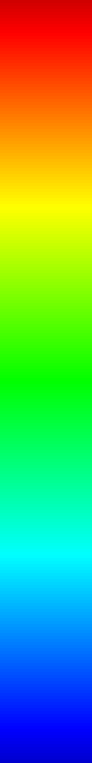
\includegraphics[angle=270, width=\linewidth, totalheight=1em, frame]{./content/pictures/rainbow.png}
			  \caption{Rainbow colormapping indicating the color from low values (left) to high values (right)}
			\end{figure}
			\item[Grayscale] ~\\ 
			The grayscale colormap is another well-known colormap. 
			It maps every value in the dataset to a value representing a gray hue, typically between 0 and 255. 
			It is quite easy to implement in RGB space (R = G = B = value) and in HSV space (H = 0, S = 0, V = value).
			\begin{figure}[htb]
			  \centering
			  
\includegraphics[angle=270, width=\linewidth, totalheight=1em, frame]{./content/pictures/black_white.png}
			  \caption{Grayscale colormapping indicating the color from low values (left) to high values (right)}
			\end{figure}
			\item[Banded] ~\\
			 This colormap is similar to the rainbow colormap as described above, but in this colormap several contiguous scalar values are assigned the same color. 
			\begin{figure}[htb]
			  \centering
			  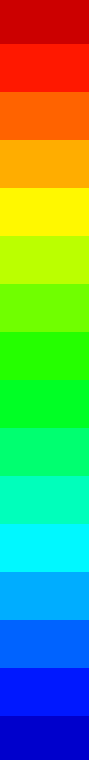
\includegraphics[angle=270, width=\linewidth, totalheight=1em, frame]{./content/pictures/rainbow_16.png}
			  \caption{Rainbow colormap with discontinuities due to banding.}
			\end{figure}
		\end{description}
		\clearpage
		These options are, however, somewhat limited. 
		To give users more options and to make the dataset more insightful for easier inverse mapping of the dataset and aesthetics, we have implemented more color maps:
		\begin{description}
			\item[Bipolar] ~\\
			The bipolar color map is a continuous diverging colormap between two colors. 
			At each end of the spectrum there is one color and colors for intermediate values is a linear interpolation of the two. 
			Because there is only a variation in hue and not in saturation or value this colormap is arguably better than a rainbow colormap.
			The end colors are customizable by the user and can therefore also be helpful for people with deuteranope or protanopic vision.\cite{moreland2009diverging}
			\begin{figure}[htb]
			  \centering
			  
\includegraphics[angle=270, width=\linewidth, totalheight=1em, frame]{./content/pictures/bipolar.png}
			  \caption{A possible bipolar colormapping indicating the color from low values (left) to high values (right)}
			\end{figure}

			\item[Zebra] ~\\
			The zebra colormap seems to be opposite of color mapping best practices: Little variance in color and several distinct and far apart values are mapped to the same color. 
			It turns out that, however unintuitive it may seem, the zebra colormap is useful. 
			The width of the bands are an indication of change in the scalar dataset values. 
			Small and frequent bands correspond to areas with high change, and areas with wide bands are subject to little change.
			In other words, the zebra colormap represents the magnitude of the gradient \(\mid\mid\nabla f\mid\mid\) of the scalar dataset\cite[p. 156]{telea2014data}
			\begin{figure}[htb]
			  \centering
			  
\includegraphics[angle=270, width=\linewidth, totalheight=1em, frame]{./content/pictures/zebra_16.png}
			  \caption{A zebra colormap consisting of 16 bands. }
			\end{figure}
		\end{description}

		We have added in GLUI a dropdown menu that lets users select one of the aforementioned colormaps and is then applied in real-time to the scalar dataset, including the option to select the number of bands.
	\subsection{Color legend}
		For colormapping, it is crucial to be able to make the inverse mapping. 
		That is, be able to see a color in your dataset and be able to tell to which value it corresponds. 
		To ease this process, we have implemented a color legend at the edge of the screen. 
		It shows all the colors of the colormap could display alongside at least three and at most ten reference values to ease the mental interpolation. 
		We have chosen for a maximum of 10 values because at this value, the total numbers displayed remains clear and fits on nearly all resolutions, while remaining detailed enough for mental value interpolation.
		% The legend for the color map has been implemented.
		% On the side of the GLUT subwindow, the reference color map is drawn with the values corresponding to the colors next to it.
	\subsection{More datasets for color map}
		In the skeleton application, only one scalar dataset, the density of the matter which flows in the vector field, was available for visualization. 
		While this is very interesting on its own, there are several other scalar datasets either readily available for visualization or can be derived from the vector field.
		
		We provided the means to choose the dataset on which color mapping can be applied.
		The function \texttt{draw\_smoke} receives a pointer to an array containing the values of the dataset that needs to be visualized.
		There are three different datasets that this pointer can reference:
		\begin{itemize}
			\item Force magnitude
			\item Velocity magnitude
			\item Fluid density
		\end{itemize}
		In case of velocity magnitude visualization, the magnitude of a vector \(a\) is determined by the following equation:
		\[\| a \|\ = \sqrt{a_x^2 + a_y^2}\]
		In case of fluid density, the existing reference to \texttt{rho} in the model can be used.
		%misschien plaatjes?
	\subsection{Scaling \& clamping}
		By default, the values of the colormap are clamped between 0.0 and 1.0. 
		This means that any value higher than 1.0 will be the color at the higher clamp value and vice versa for values lower than 0.0.
		While this could work in practice, it is desirable to have the option to modify this displaying behavior because datasets as the divergence or the fluid velocity are about very small values whose meaning would disappear if default clamping is used.

		Therefore we have made two modifications to the value display options:
		Firstly, we have modified the ranges of clamping values from their default range \([0, 1]\) to an user settable \texttt{min} and \texttt{max}. 
		This makes it possible to use clamping when the values of the scalar dataset are very small or very large.

		Secondly, we have implemented scaling behavior. 
		In this option the scale values \texttt{min} and \texttt{max} are set to respectively the lowest and the highest values in the scalar dataset. 
		This causes that all colors in the dataset are relative to the respective colors of the minimum value and the maximum value of the dataset which is an intuitive way to display a scalar dataset.
	\subsection{Limit number of colors}
		By default, 256 different colors are used in a dataset. 
		This provides a diverse and gradual amount of colors which can be mapped onto a dataset.
		However, it is sometimes desirable to use fewer colors because, for example, an user is not interested in small differences between neighboring values.

		To achieve this, we have implemented color banding. 
		A value can be set which corresponds to the number of colors which can be used from a color map.
		The available colors are chosen uniformly over the entire range of colors.
		The results are visible in figures~\ref{fig:rainbow} and~\ref{fig:rainbow_banded}.
		The difference between limited color banding and the default color banding can be seen in Figure~\ref{fig:banded_difference}.
		\begin{figure}[htb]
			  \centering
			  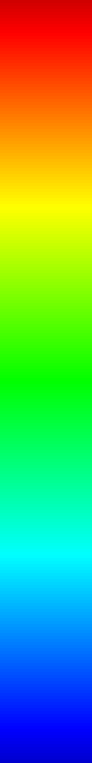
\includegraphics[angle=270, width=\linewidth, totalheight=1em, frame]{./content/pictures/rainbow.png}
			  \caption{A rainbow colormap with no colorbanding. Therefore it has 256 different "boxes" which we perceive as a continuous. }
			  \label{fig:rainbow}
		\end{figure}
		\begin{figure}[htb]
			  \centering
			  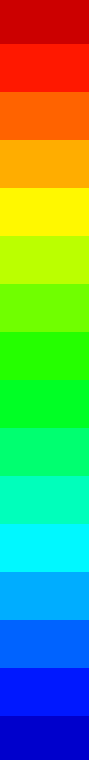
\includegraphics[angle=270, width=\linewidth, totalheight=1em, frame]{./content/pictures/rainbow_16.png}
			  \caption{The same rainbow colormap banded to 16 colors. A boxing effect is visible which could be useful.}
			  \label{fig:rainbow_banded}
		\end{figure}
		\begin{figure}[htb]
			  \centering
			  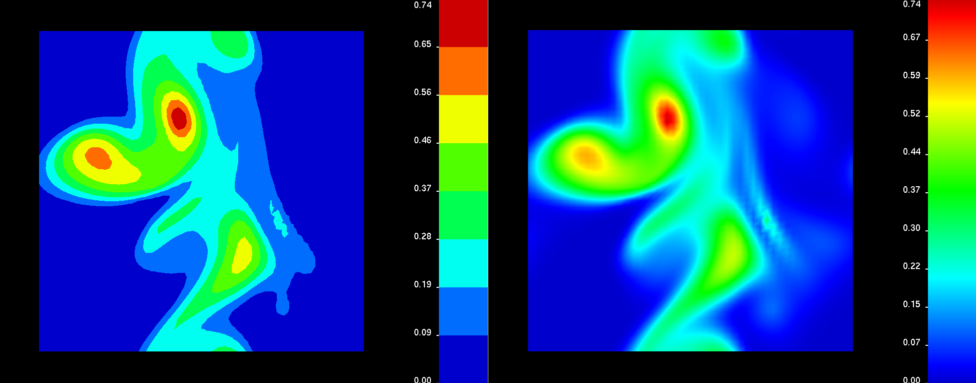
\includegraphics[width=\linewidth]{./content/pictures/limit_colors.png}
			  \caption{Limited color banding at work.}
			  \label{fig:banded_difference}
		\end{figure}

	\subsection{HSV color space}
		Generally, humans are not good at manipulating colors in the \texttt{RGB}-space. 
		When a user is asked for the \texttt{RGB}-value of red (\texttt{\#ff0000}) at 50\% saturation and a brightness of 75\%, people will generally not be able to tell the corresponding \texttt{RGB}-value (\texttt{\#bf5f5f}).
		To make this process more natural for human perception, we have added the option to manipulate colors in HSV space, which is a mapping of the RGB colorspace to define it in terms of hue, saturation and value (or brightness).
		Controls are added to manipulate the saturation and value, both ranging from 0\% to 100\%.
		For this, we used the conversion function from RGB to HSV and vice versa, as described in \cite{telea2014data}.
	\subsection{1D textures}
		The entire simulation is run on a grid.
		By default, smooth shading is used, meaning the colors of the vertices of objects are interpolated over the surface areas of objects.
		It is a fast and acceptable model, but it does not allow for discontinuous color bands which can be present in the simulation.
		To overcome this problem we have implemented 1D texture mapping.
		In this model, the colormap is stored in OpenGL as a 1-dimensional texture of all possible colors.
		When a surface is drawn in OpenGL, the texture is mapped to it which results in per-pixel interpolation color mapping according to the colors stored in the textures. 
		This allows for discontinuous bands within surfaces, making the entire application more useful and aesthetically pleasing.
		The effects are visible in figures~\ref{fig:without_textures} and~\ref{fig:with_textures}.
		\begin{figure}[htb]
			  \centering
			  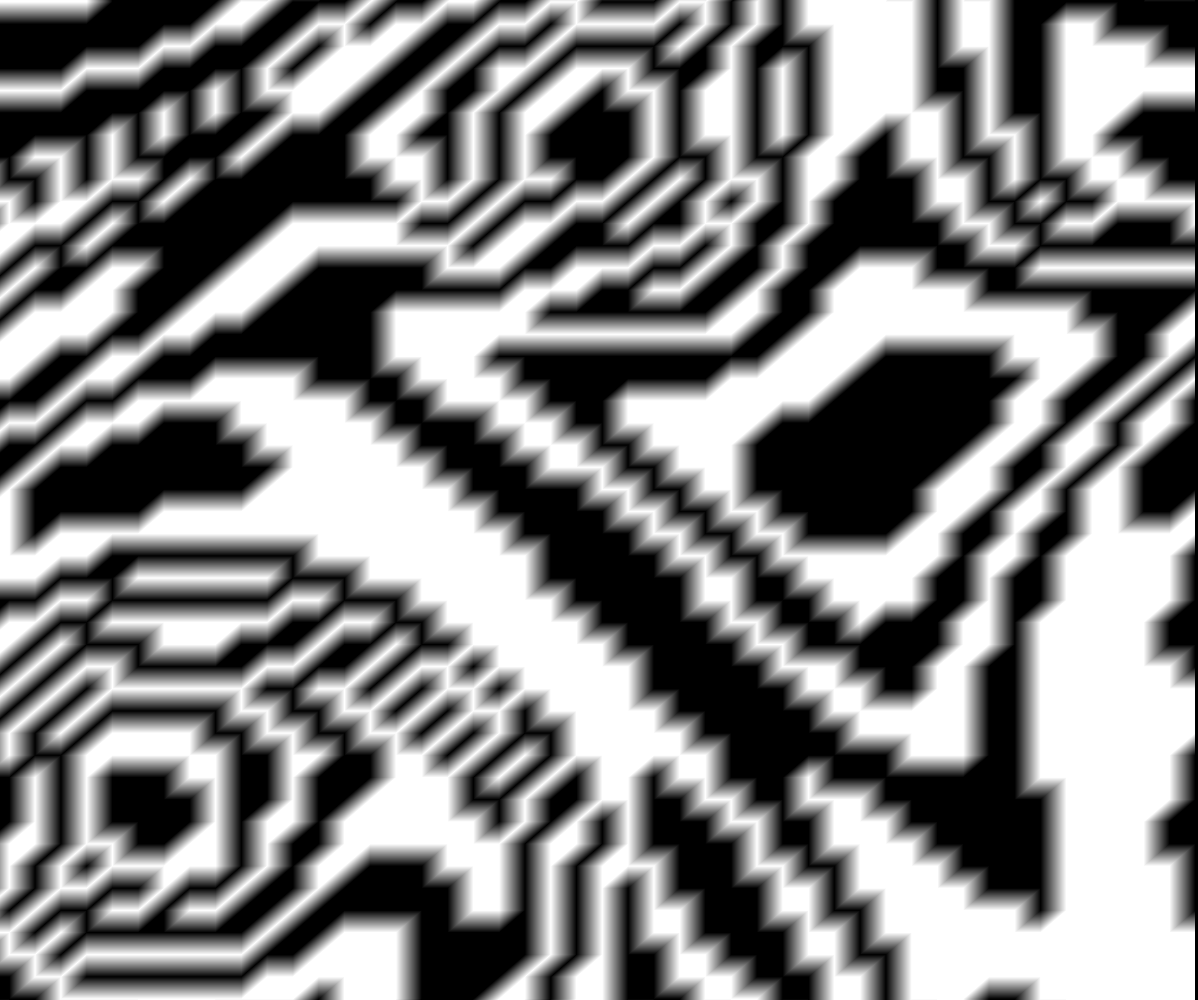
\includegraphics[scale=.2]{./content/pictures/zebra_regular.png}
			  \caption{The zebra colormap applied to a dataset without texture mapping. Its usability is limited.}
			  \label{fig:without_textures}
		\end{figure}
		\begin{figure}[htb]
			  \centering
			  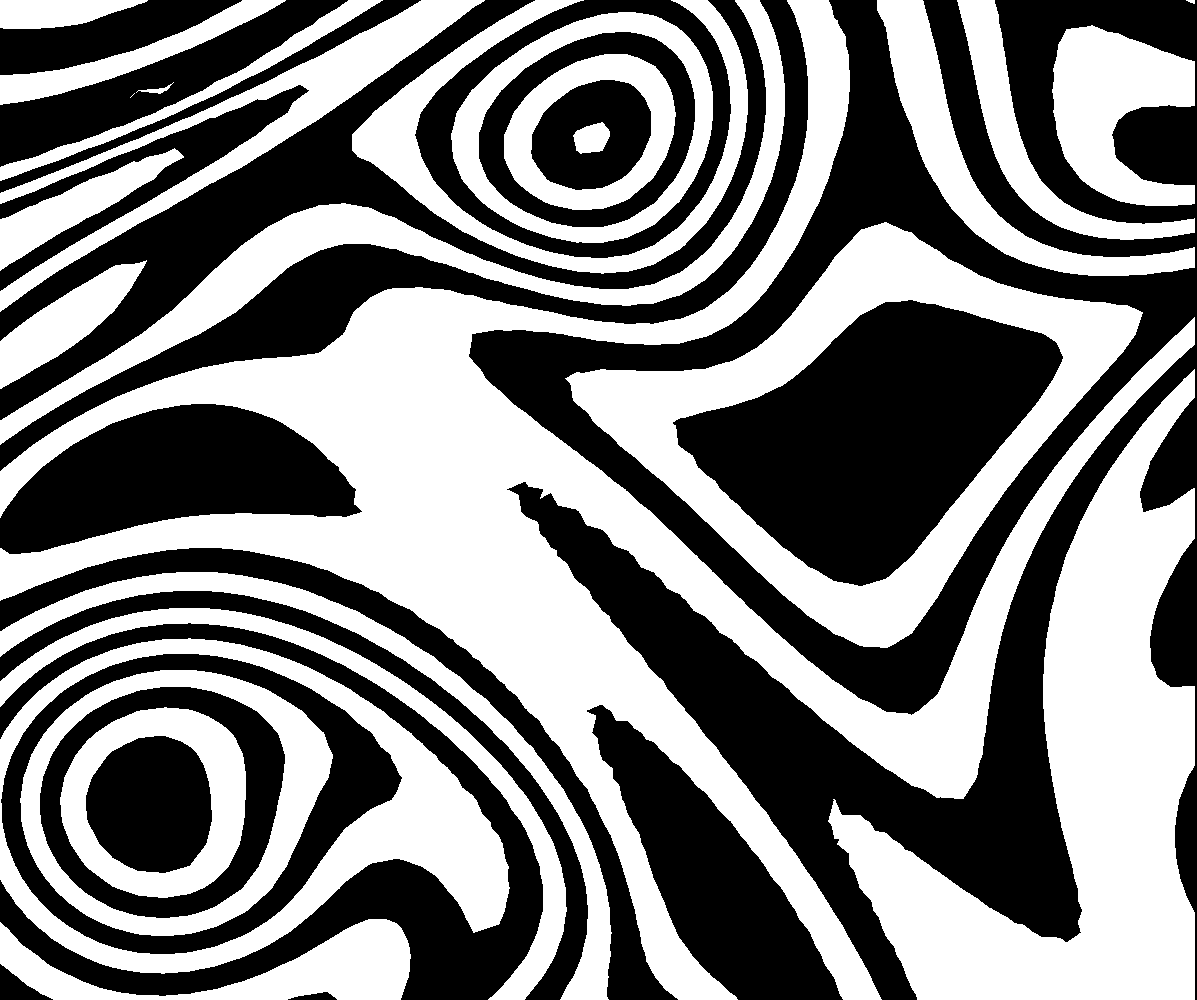
\includegraphics[scale=.2]{./content/pictures/zebra_texture.png}
			  \caption{The zebra colormap applied to the same dataset with texture mapping. The image is clearer and more useful.}
			  \label{fig:with_textures}
		\end{figure}

\clearpage